\documentclass[xcolor={usenames,dvipsnames}]{beamer}
\usepackage[utf8]{inputenc}
\usepackage[english]{babel}

% -- Including some standard packages --
\usepackage{graphicx}
\usepackage{soul}
\usepackage{hyperref}
\usepackage{colortbl}
\usepackage{dsfont}
\usepackage{soul}

% -- Choosing theme --

\usetheme{Boadilla}
\usecolortheme{spruce}
\setbeamercolor{alerted text}{fg=purple} % Making alerted text non-red

% Tikz
\usepackage{tikz,tikz-3dplot,tikz-cd,tkz-tab,tkz-euclide,pgf,pgfplots}
\usetikzlibrary{matrix,positioning,fit,backgrounds,intersections}

% -- Cross signs --
\usepackage{pifont} % http://ctan.org/pkg/pifont
\newcommand{\cmark}{\ding{51}}%
\newcommand{\xmark}{\ding{55}}%
\newcommand{\xopt}{\ding{48}}%

% -- Custom commands --
\DeclareMathOperator*{\argmax}{arg\,max}
\DeclareMathOperator*{\argmin}{arg\,min}

\title[Commitment schemes]{\textbf{Commitment schemes}}
\author{Distributed Lab}
\date{August 20, 2024}
\titlegraphic{
    
\includegraphics[width=\textwidth]{images/banner_wide.png}
}

\expandafter\def\expandafter\insertshorttitle\expandafter{%
  \insertshorttitle\hfill%
  \insertframenumber\,/\,\inserttotalframenumber}

\AtBeginSection[]{
  \begin{frame}
  \vfill
  \centering
  \begin{beamercolorbox}[sep=8pt,center,shadow=true,rounded=true]{title}
    \usebeamerfont{title}\insertsectionhead\par%
  \end{beamercolorbox}
  \vfill
  \end{frame}
}

\begin{document}
	\frame {
		\titlepage
	}
 
	\begin{frame}{Plan}
        \tableofcontents
    \end{frame}

	\section{Commitments Overview}

    \begin{frame}{Commitment Definition}
        \begin{definition}
            A cryptographic commitment scheme allows one party to commit to a chosen statement without revealing the statement itself. 
            The commitment can be revealed in full or in part at a later time, ensuring the integrity and secrecy of the original statement until 
            the moment of disclosure.
        \end{definition}

        \begin{figure}
            \centering
            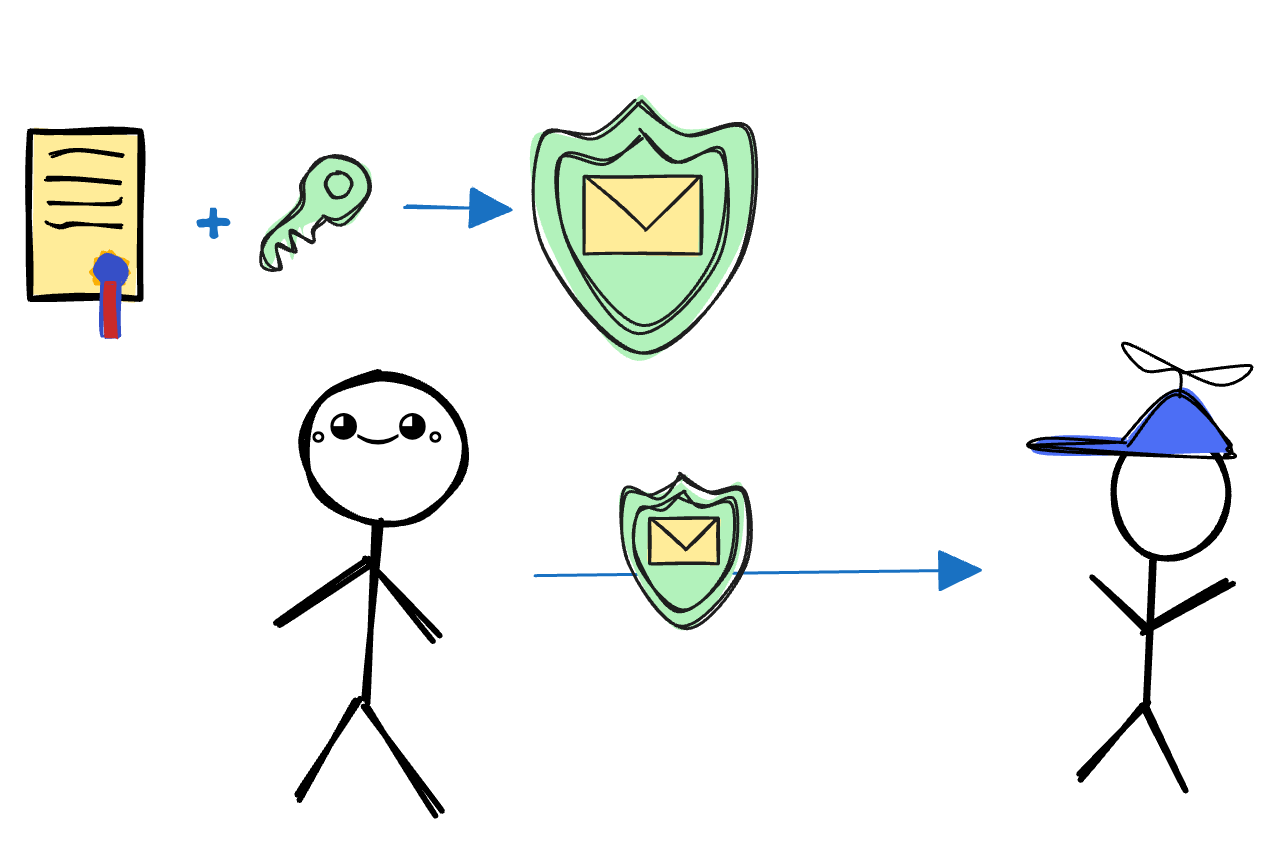
\includegraphics[width=0.5\textwidth]{images/lecture_5/CommitmentExample.png}
            \caption{Overview of a commitment scheme}
        \end{figure}
    \end{frame}

    \begin{frame}{Commitment Definition}
        \begin{definition}
            Commitment Scheme $\Pi_{\text{commitment}}$ is a tuple of three algorithms: $\Pi_{\text{commitment}} = (\mathsf{Setup}, \mathsf{Commit}, \mathsf{Verify})$.

            \begin{enumerate}

                \item Setup ($1^{\lambda}$): returns public parameter \textit{pp} for both comitter and verifier;

                \item  Commit ($\mathsf{pp}, m, r$): returns a commitment $c$ to the message $m$ using public parameters \textit{pp} and, optionally, a secret opening hit $r$;

                \item  Open ($\mathsf{pp}, c, m, r$): verifies the opening of the commitment to the message $m$ with an opening hit $r$. 
            \end{enumerate}
        \end{definition}

    \end{frame}

    \begin{frame}{Commitment Scheme Properties}
        \begin{definition}
            \begin{enumerate}
                \item \textit{Hiding: } verifier should not learn any additional information about the message given only the commitment $\mathcal{C}$.
                \begin{enumerate}
                    \item \textit{Perfect hiding}: adversary with any computation capability tries even forever cannot understand what you have hidden.
                    \item \textit{Computationally hiding}: we assume that the adversary have limited computational resources and cannot try forever to recover hidden value.
                \end{enumerate}
                
                \item \textit{Binding: } prover could not find another message $m_1$ and open the commitment $\mathcal{C}$ without revealing the commited message $m$.
                \begin{enumerate}
                    \item \textit{Perfect binding}: adversary with any computation capability tries even forever cannot find another $m_1$ that would result to the same $\mathcal{C}$.
                    \item \textit{Computationally binding}: we assume that the adversary have limited computational resources and cannot try forever.
                \end{enumerate}
            \end{enumerate}
        \end{definition}
        \begin{alertblock}{Note}
            Perfect hiding and perfect binding cannot be achived at the same time
        \end{alertblock}    
    \end{frame}

    \section{Hash-based Commitments}

    \begin{frame}{Hash-based commitments}

        As the name implies, we are using a cryptographic hash function \(H\) in such scheme.

        \begin{definition}
            \begin{enumerate}
                \item Prover selects a message $m$ from a message space $M$ which he wants to commit to:
                    $m \leftarrow \mathbb{M}$
            
                \item Prover samples random value $r$ from a challange space $C$ (usually called blinding factor) from $\mathbb{Z}$:
                    $r \xleftarrow{R} \mathbb{C}$
                
                \item Both values will be concatenated and hashed with the hash function $H$ to produce the commitment:
                    $\mathcal{C} = H(m \parallel r)$
            \end{enumerate}
        \end{definition}

    \end{frame}

    \section{Vector Commitments}

    \subsection{Merkle Tree based Vector Commitment}

    \begin{frame}{Merkle Tree commitments}

        A naive approach for a vector commitment would be hash the whole vector. 
        More sophisticated scheme uses divide-and-conquer approach by building a binary tree out of vector elements.

        \begin{figure}
            \centering
            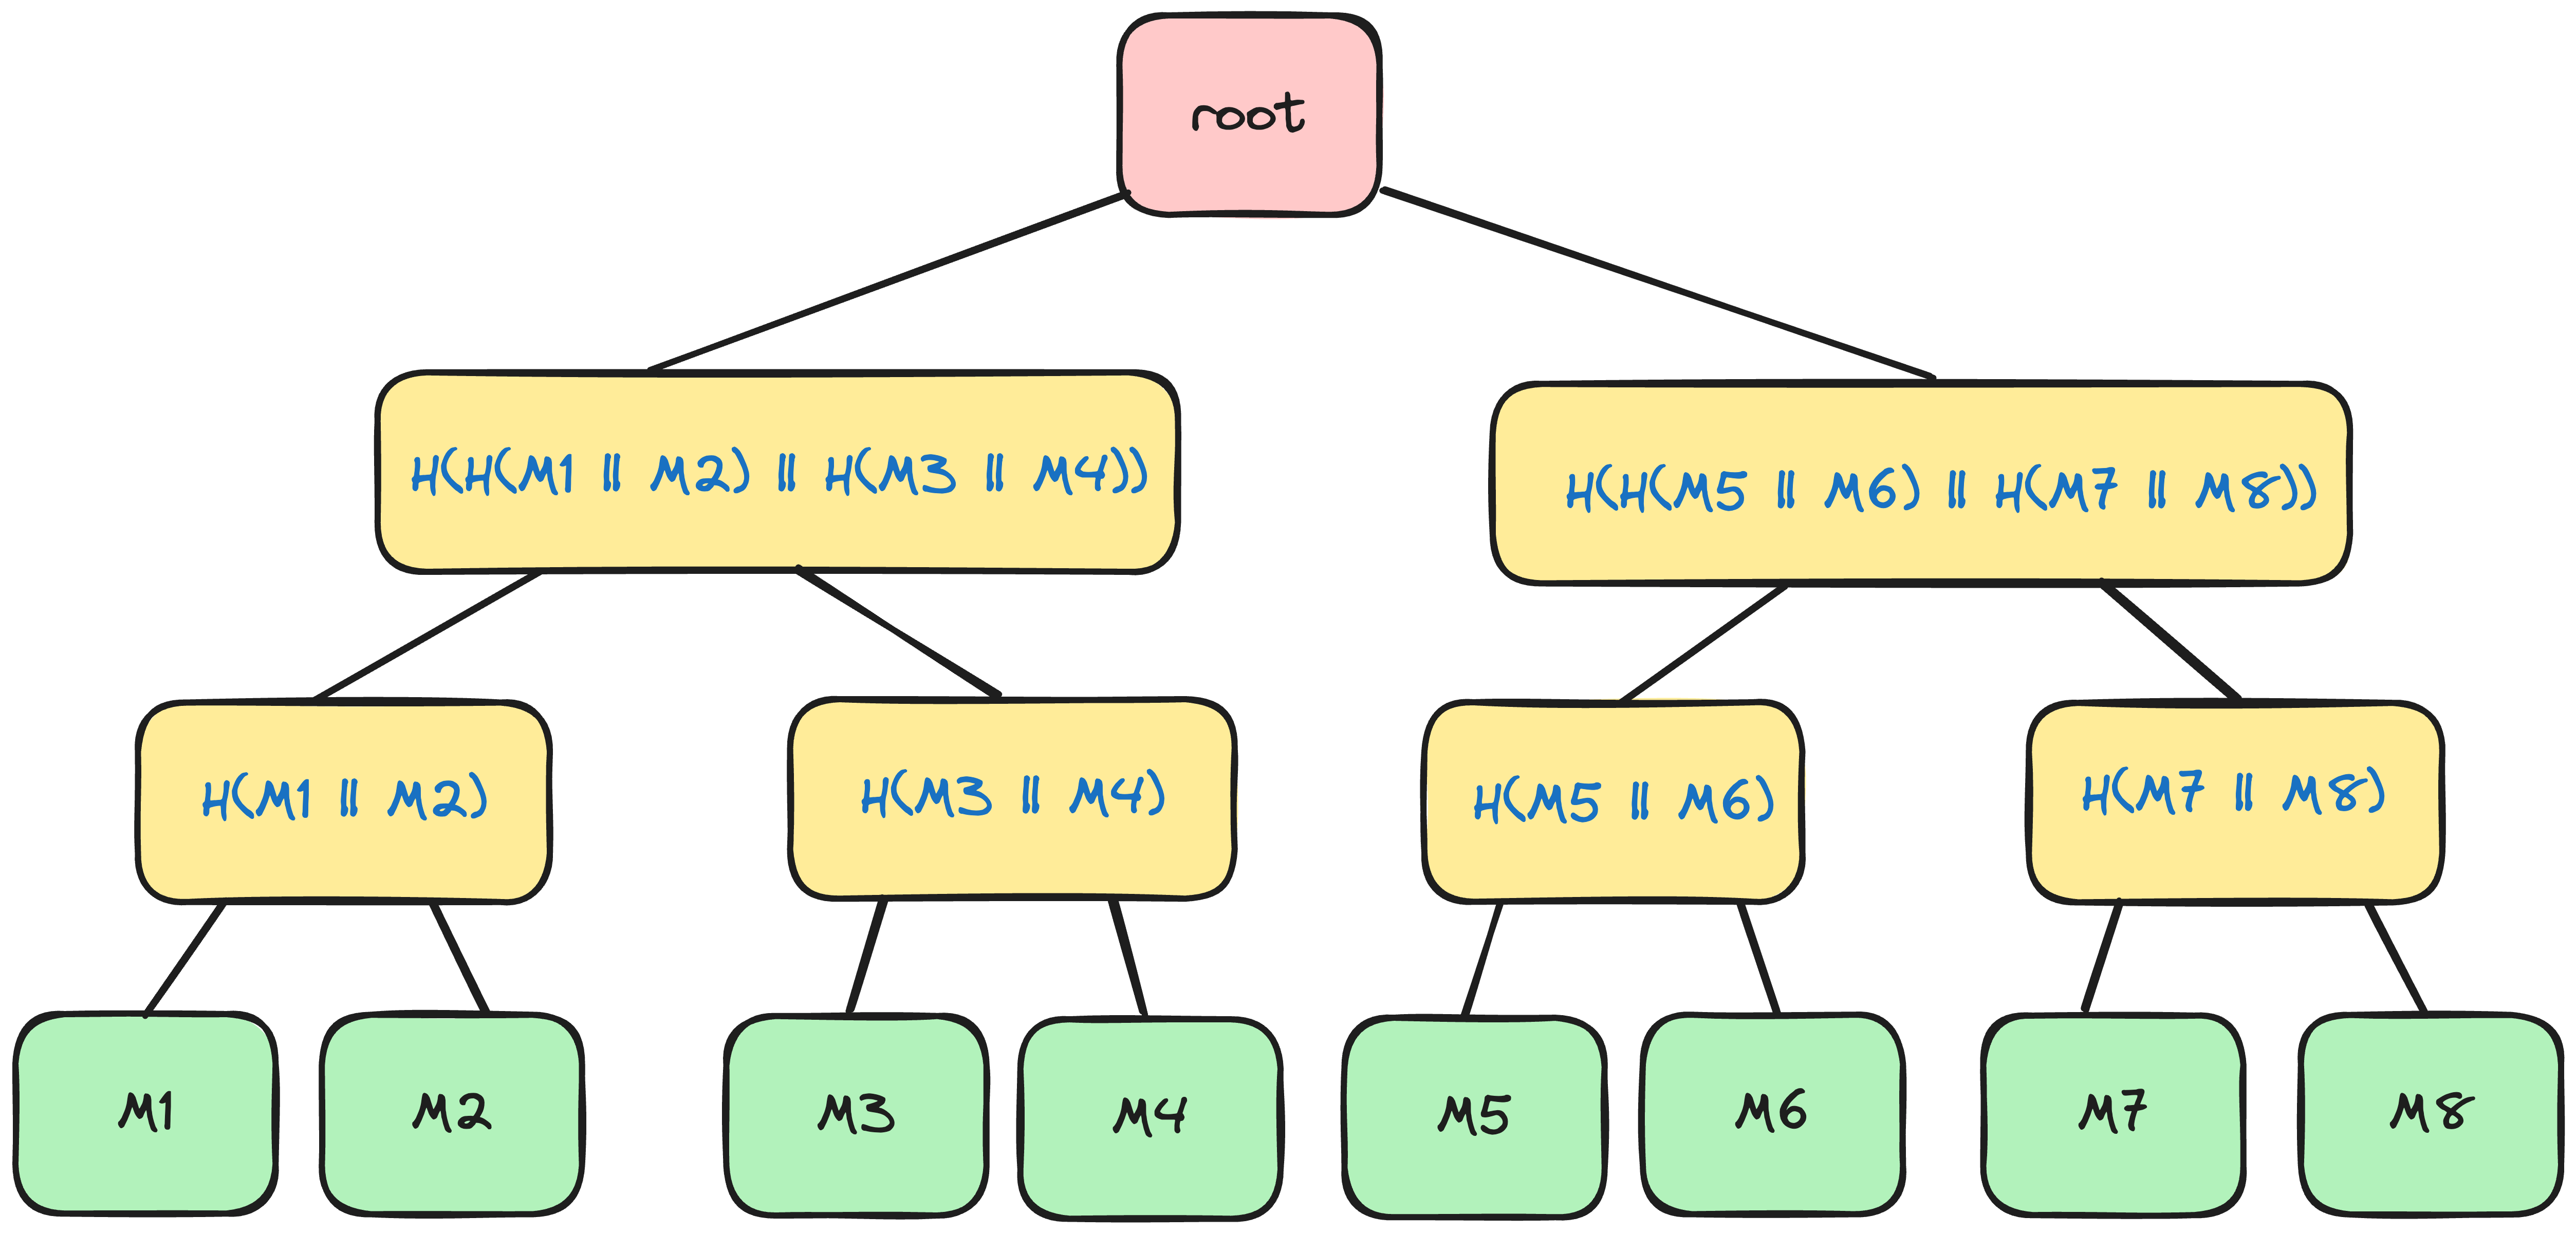
\includegraphics[width=0.75\textwidth]{images/lecture_5/MerkleTree.png}
            \caption{Merkle Tree structure}
        \end{figure}

    \end{frame}

    \begin{frame}{Merkle Tree Proof (MTP)}

        To prove the inclusion of element into the tree, a corresponding Merkle Branch is used. It allows to perform selective
        disclosure of the elements without revealing all of them at once.

        \begin{figure}
            \centering
            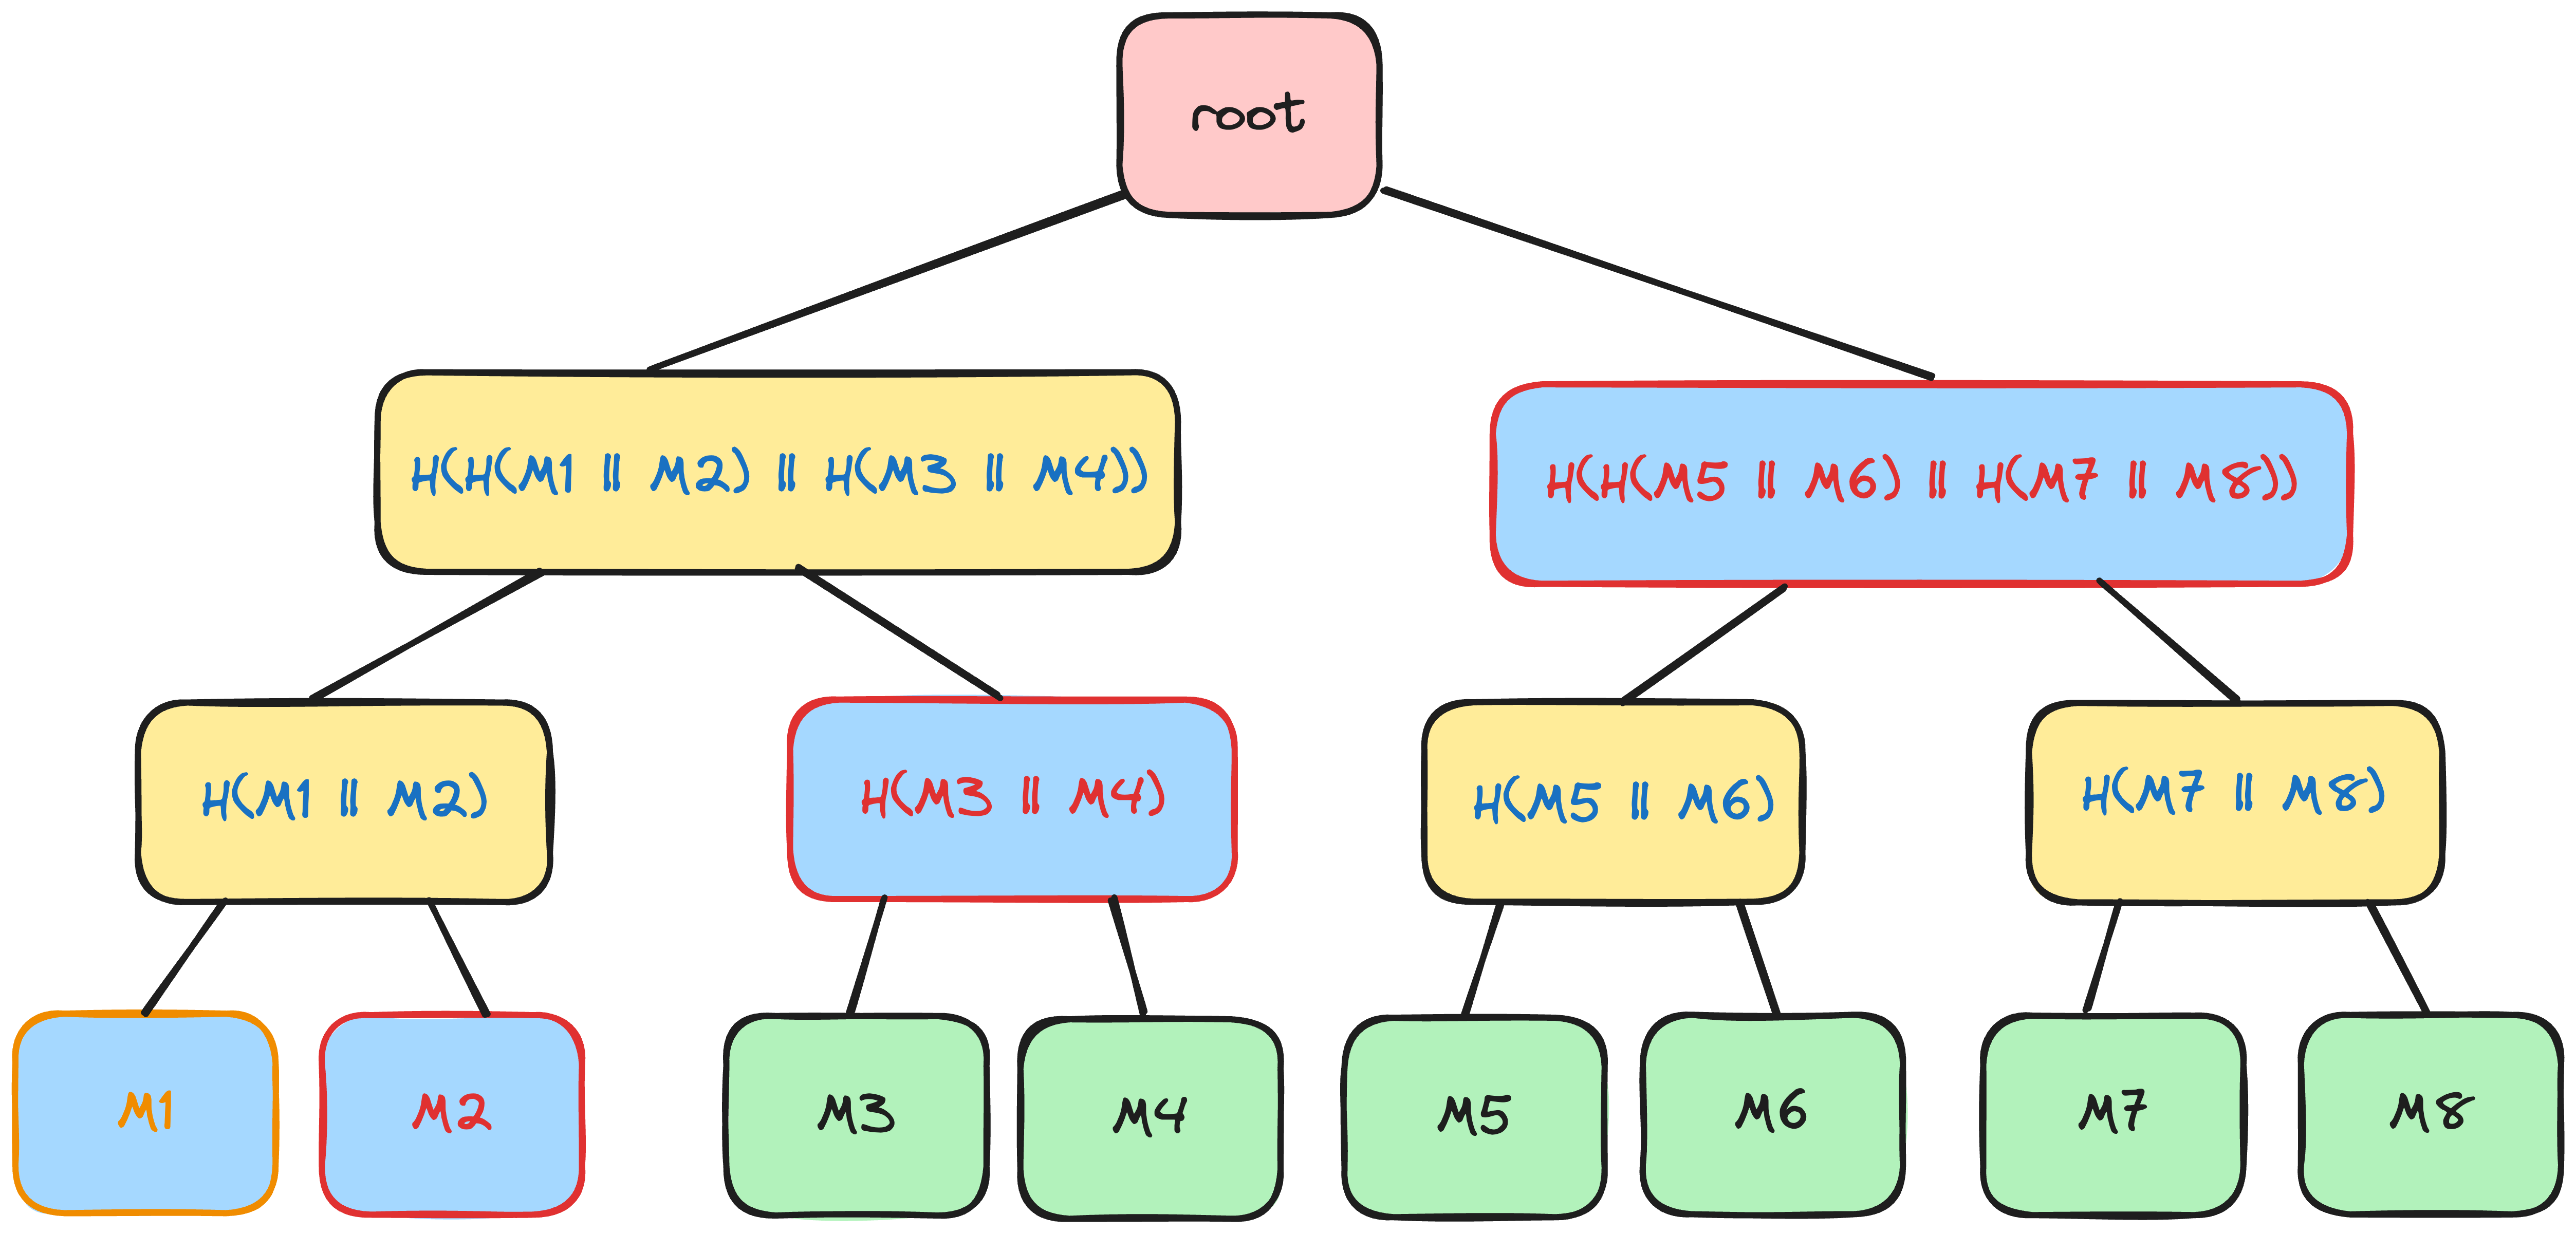
\includegraphics[width=0.75\textwidth]{images/lecture_5/MerkleTreeProof.png}
            \caption{Merkle Tree inclusion proof branch}
        \end{figure}

    \end{frame}

    \subsection{Pedersen commitment}

    \begin{frame}{Pedersen Commitment}

        Pedersen commitments allow us to represent arbitrarily large vectors with a single elliptic curve point. 
        Pedersen commitment uses a public group $\mathbb{G}$ of order $q$ and two random public generators
        $G$ and $U$: $U = [u]G$. Secret parameter $u$ should be unknown to anyone, otherwise the $\textit{Binding}$ 
        property of the commitment scheme will be violated.
    
        \begin{alertblock}{Note: Transparent random points generation}
            User can pick the publicly known number (like $x$ coordinate of group generator $G$), calculate $x_i = H(x \parallel i)$
            and corresponding $y_i$. Check whether $(x_i, y_i)$ is in the elliptic curve group. Repeat the process for sequential $i = 1, 2 \ldots$
            until point $(x_i, y_i)$ is in the elliptic curve group.
        \end{alertblock}    

    \end{frame}

    \begin{frame}{Pedersen Commitment}

        \begin{definition}
            Pedersen commitment scheme algorithm:
            \begin{enumerate}
                \item Prover and Verifier agrees on $G$ and $U$ points in a elliptic curve point group $\mathbb{G}$, $q$ is the order of the group.
                \item Prover selects a value $m$ to commit and a blinder factor $r$:
                        $m \leftarrow \mathbb{Z}_q$,
                        $r \xleftarrow{R} \mathbb{Z}_q$
                \item Prover generates a commitment and sends it to the Verifier:
                        $\mathcal{C} \gets [m]G + [r]U$
            \end{enumerate}
        \end{definition}

        During the opening stage, prover reveals $(m, r)$ to the verifier. 
        
        To check the commitment, verifier computes: $\mathcal{C}_1 = [m]G + [r]U$. 
        
        If $\mathcal{C}_1 = \mathcal{C}$, prover has revealed the correct pair $(m, r)$.

    \end{frame}

    \begin{frame}{Pedersen Commitment}

            In case the discrete logarithm of $U$ is leaked, the \textit{binding} property can be violated by the \textit{Prover}:
        
            \begin{center}
                $c = [m]G + [r]U = [m] G + [r \cdot u]G = [m + r \cdot u] G$
            \end{center}
        
            For example, $(m + u, r - 1)$ will have the same commitment value:
        
            \begin{center}
                $[m+u + (r-1) \cdot u] G = [m + u - u + r \cdot u] G = [m + r \cdot u] G$     
            \end{center}
            
    \end{frame}

    \begin{frame}{Pedersen Commitment Aggregation}

        Pedersen commitment have some advantages compared to hash-based commitments.
        Additively homomorphic property allows to accumulate multiple commitments into one.
        Consider two pairs: $(m_1, r_1), (m_2, r_2)$.
        
        \begin{center}
            $\mathcal{C}_2 = [m_1]G + [r_1]U$,
        
            $\mathcal{C}_2 = [m_2]G + [r_2]U$,
        
            $\mathcal{C}_a = \mathcal{C}_1 + \mathcal{C}_2 = [m_1 + m_2]G + [r_1 + r_2]U$
        \end{center}
        
        This works for any number of commitments, so we can encode as many points as we like in a single one.

        \begin{figure}
            \centering
            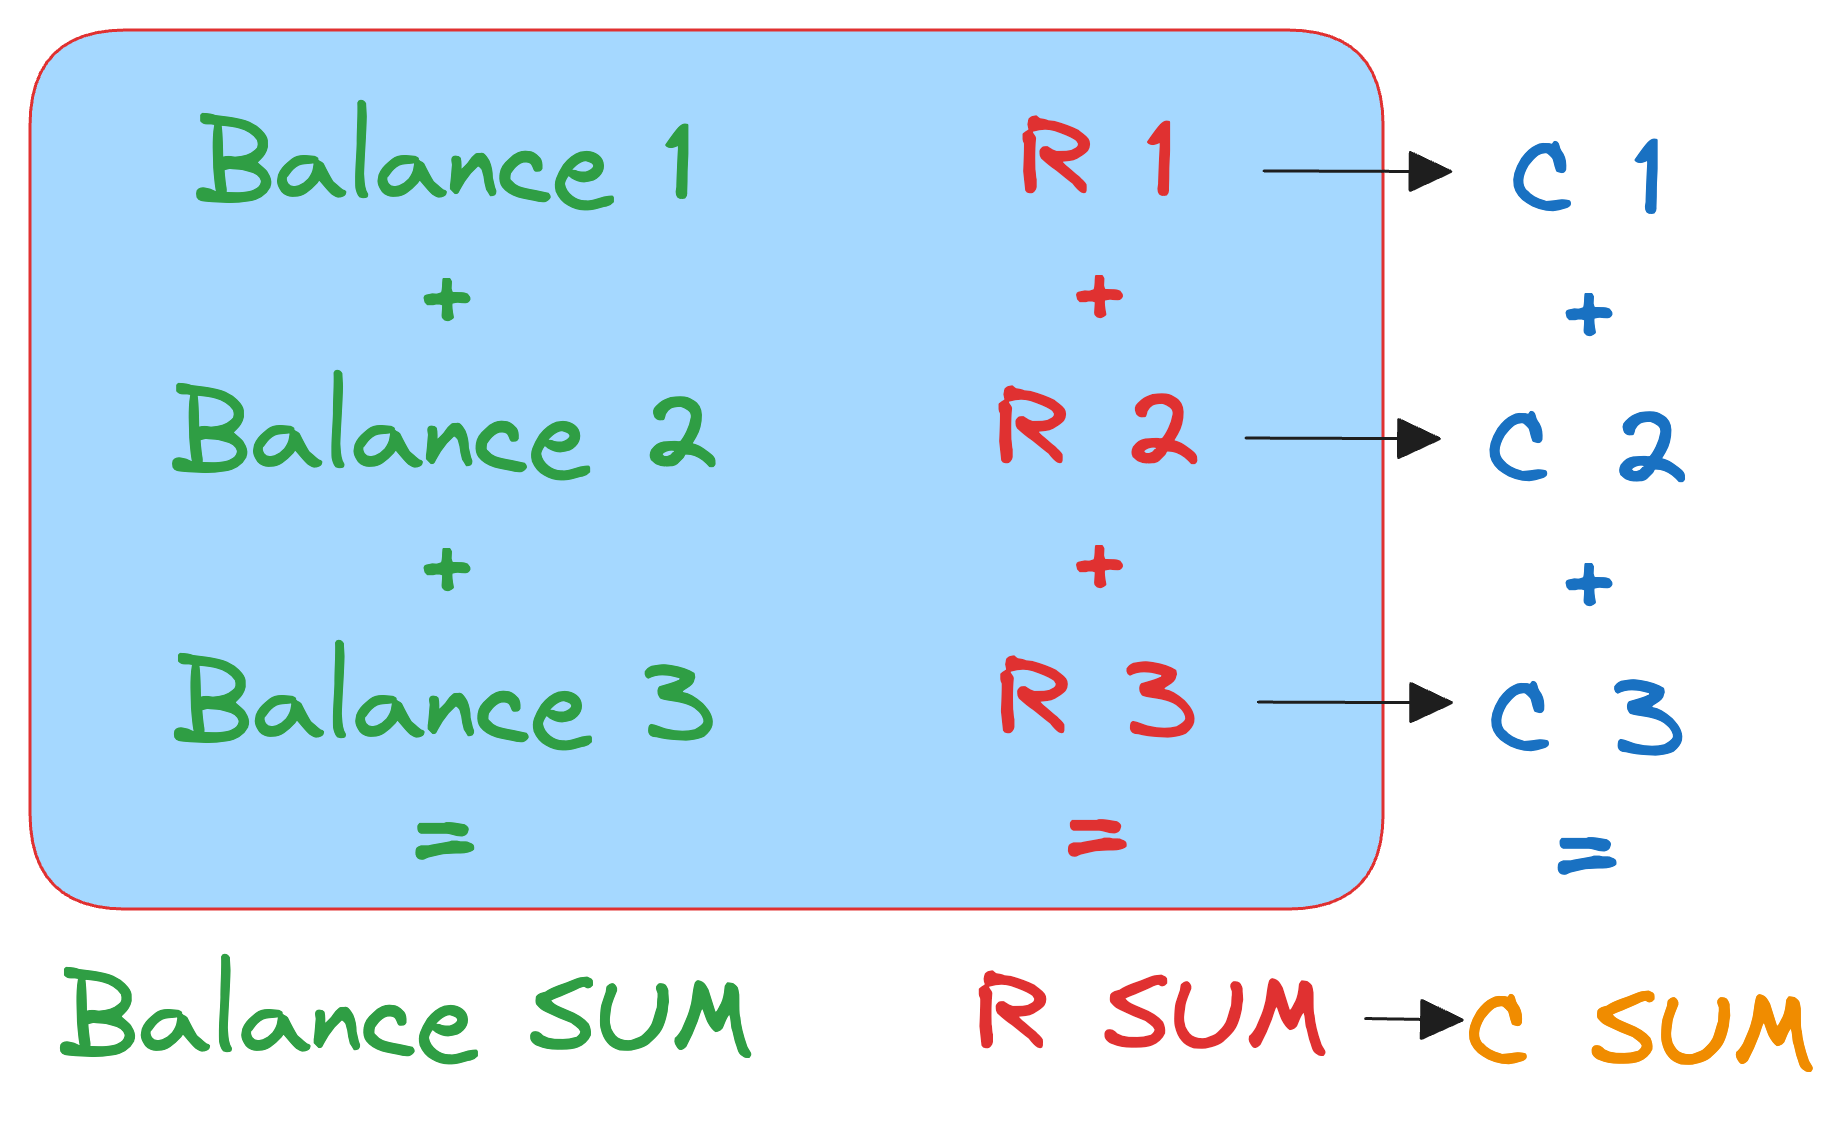
\includegraphics[width=0.4\textwidth]{images/lecture_5/Balances.png}
        \end{figure}
        
\end{frame}

    \begin{frame}{Pedersen Vector Commitment}

        Suppose we have a set of random elliptic curve points $(G_1, \ldots ,G_n)$ of cyclic group $\mathbb{G}$ 
(that nobody knows the discrete logarithm of), a vector $(m_1, m_2 \ldots m_n)$ and a random value $r$. We can do the following:

\begin{center}
    $ \mathcal{C} = m_1\cdot[G_1] + m_2 \cdot [G_2] \ldots + m_n \cdot [G_n] + r \cdot [Q]$ 
\end{center}

Since the \textit{Prover} does not know the discrete logarithm of the generators, so he can only reveal $(v_1, \ldots ,v_n)$ to produce $[C]$ later, they cannot produce another vector.

Prover can later open the commitment by revealing the vector $(m_1, m_2 \ldots m_n)$ and a blinding term $r$.

        
\end{frame}


    
	\begin{frame}{}
      \centering \Large
      \emph{Thanks for your attention!}
    \end{frame}
\end{document}